\section{Desempeño de ordenamiento}
La Tabla~\ref{tab:main-results} resume la comparación de modelos. Las líneas base triviales se comportan como se esperaba: ROC AUC permanece en el nivel del azar y PR AUC se mantiene cerca de la prevalencia positiva de aproximadamente $0.726$. Esto proporciona una referencia útil sin capacidad predictiva y respalda la consistencia interna de la evaluación.

Entre los modelos no triviales, TF--IDF más regresión logística obtiene las mejores métricas de ordenamiento, con ROC AUC medio de $0.814$ y PR AUC medio de $0.899$. El transformer entre fragmentos aplicado a embeddings de LLM alcanza ROC AUC de $0.755$ y PR AUC de $0.886$. Las líneas base con embeddings promediados se mantienen próximas: el MLP con promedio alcanza ROC AUC de $0.763$ y PR AUC de $0.894$, mientras que la regresión logística con promedio alcanza ROC AUC de $0.758$ y PR AUC de $0.881$. La Fig.~\ref{fig:pr} coincide con este panorama: TF--IDF define en general la mejor frontera entre precisión y exhaustividad, mientras que ambas alternativas basadas en LLM permanecen claramente por encima de la prevalencia. Los documentos contienen señal predictiva, pero el mejor ordenamiento en la configuración actual proviene de representaciones léxicas y no densas.

\section{Sensibilidad al umbral}
El comportamiento dependiente del umbral revela un patrón diferente. Con el umbral predeterminado de $0.5$, el transformer entre fragmentos alcanza el mayor F1 ($0.858$ en la evaluación original de cinco pliegues). Sin embargo, el experimento específico muestra que no todos los modelos reaccionan de igual manera a la optimización del umbral. Para TF--IDF más regresión logística, seleccionar en validación el umbral que maximiza F1 incrementa el F1 del pliegue de prueba en $0.103$ en promedio, pero no mejora la exactitud balanceada media. La regresión logística con promedio presenta una mejora modesta de F1 ($+0.014$) y una disminución media de exactitud balanceada ($-0.049$). En contraste, el transformer cambia poco con el ajuste (media de $\Delta$F1 $=+0.002$ y media de $\Delta$ de exactitud balanceada $=+0.002$), lo que indica que el umbral predeterminado ya está cerca de un punto operativo estable. El MLP con promedio ocupa una posición intermedia: su F1 apenas cambia, pero su exactitud balanceada mejora en promedio al ajustar el umbral. La Fig.~\ref{fig:threshold-sensitivity} resume visualmente el contraste y deja claro que la optimización beneficia principalmente el F1 del modelo léxico, no a todos los modelos de manera uniforme.

\section{Calibración}
La calibración presenta una historia diferente al ordenamiento. El transformer entre fragmentos consigue el mejor puntaje de Brier ($0.162$), seguido por el MLP con promedio ($0.165$); TF--IDF más regresión logística obtiene un resultado inferior ($0.179$) y la regresión logística con promedio es considerablemente peor ($0.201$). Este patrón indica que las características léxicas pueden ser muy eficaces para ordenar ejemplos, mientras que las representaciones densas basadas en LLM proporcionan probabilidades más confiables. La Fig.~\ref{fig:calibration} concuerda con esta interpretación: entre las tres familias más informativas, el transformer permanece más próximo a la diagonal en gran parte del intervalo de probabilidades, mientras que TF--IDF es mejor en ordenamiento que en calibración. Esto importa porque la selección de modelos para monitorear contrataciones puede depender no solo del ordenamiento, sino también de si las probabilidades permiten sustentar la priorización posterior o una puntuación de riesgo \cite{silvafilho2023calibration}.

\section{Comparación de representaciones}
La comparación entre embeddings promediados y el transformer entre fragmentos es informativa por sí misma. Si el valor principal de la representación del LLM proviniera únicamente de las interacciones entre fragmentos, cabría esperar que el transformer dominara las líneas base con promedio. Esto no sucede. El MLP con promedio supera ligeramente al transformer en ROC AUC y PR AUC, mientras que la regresión logística con promedio logra una exactitud balanceada considerablemente mayor. Los resultados sugieren que gran parte de la información predictiva ya está codificada en los propios embeddings congelados y que el modelado explícito entre fragmentos ofrece ganancias limitadas en la configuración actual. La principal ventaja del transformer parece ser la calibración y la estabilidad del umbral, no un ordenamiento claramente superior.

\begin{table}[t]
\centering
\caption{Comparación de modelos mediante validación cruzada de cinco pliegues (media $\pm$ desviación estándar). Un valor menor es mejor para Brier; un valor mayor es mejor para las demás métricas.}
\label{tab:main-results}
\footnotesize
\begin{tabular}{>{\raggedright\arraybackslash}p{0.46\linewidth} >{\raggedleft\arraybackslash}p{0.20\linewidth}}
\toprule
Métrica & Valor \\
\midrule
Mayoría: ROC AUC / PR AUC & 0.500 / 0.726 \\
Aleatorio: ROC AUC / PR AUC & 0.493 / 0.724 \\
TF--IDF + Reg. Log.: ROC AUC / PR AUC & 0.814 / 0.899 \\
TF--IDF + Reg. Log.: F1 / Exact. Bal. / Brier & 0.790 / 0.728 / 0.179 \\
Promedio + Reg. Log.: ROC AUC / PR AUC & 0.758 / 0.881 \\
Promedio + Reg. Log.: F1 / Exact. Bal. / Brier & 0.843 / 0.704 / 0.201 \\
Promedio + MLP: ROC AUC / PR AUC & 0.763 / 0.894 \\
Promedio + MLP: F1 / Exact. Bal. / Brier & 0.849 / 0.604 / 0.165 \\
Transformer entre fragmentos: ROC AUC / PR AUC & 0.755 / 0.886 \\
Transformer entre fragmentos: F1 / Exact. Bal. / Brier & 0.858 / 0.636 / 0.162 \\
\bottomrule
\end{tabular}
\end{table}

\begin{table}[t]
\centering
\caption{Ajuste del umbral en una partición interna de validación y evaluación en el pliegue externo de prueba. Se informan las medias de todos los pliegues.}
\label{tab:thresholds}
\begin{tabular}{>{\raggedright\arraybackslash}p{0.44\linewidth} >{\raggedleft\arraybackslash}p{0.22\linewidth}}
\toprule
Métrica & Valor \\
\midrule
TF--IDF + Reg. Log.: $\Delta$F1 / $\Delta$ Exact. Bal. & $+0.103 / -0.008$ \\
Promedio + Reg. Log.: $\Delta$F1 / $\Delta$ Exact. Bal. & $+0.014 / -0.049$ \\
Promedio + MLP: $\Delta$F1 / $\Delta$ Exact. Bal. & $+0.002 / +0.053$ \\
Transformer entre fragmentos: $\Delta$F1 / $\Delta$ Exact. Bal. & $+0.002 / +0.002$ \\
\bottomrule
\end{tabular}
\end{table}

\begin{figure}[t]
  \centering
  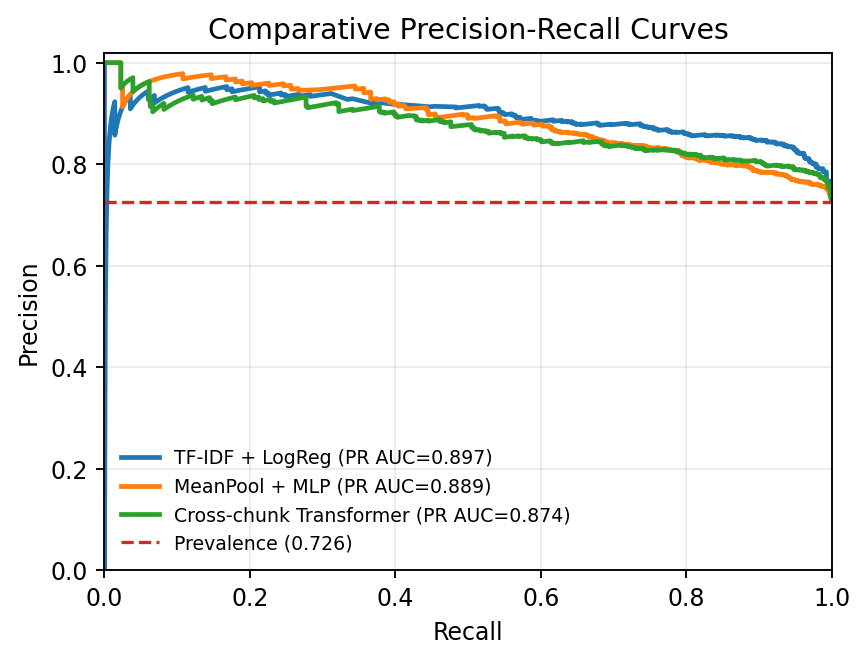
\includegraphics[width=0.94\linewidth]{figures/pr_curve_cv.png}
  \caption{Curvas comparativas de precisión-exhaustividad a partir de predicciones agregadas fuera de pliegue para la línea base léxica más sólida (TF--IDF + regresión logística), la mejor línea base densa con promedio (Promedio + MLP) y el transformer entre fragmentos. La línea horizontal discontinua marca la prevalencia positiva ($\pi \approx 0.726$). TF--IDF muestra en general el mejor compromiso entre precisión y exhaustividad, mientras que ambos modelos basados en LLM permanecen sustancialmente por encima de la referencia sin capacidad predictiva.}
  \label{fig:pr}
\end{figure}

\begin{figure}[t]
  \centering
  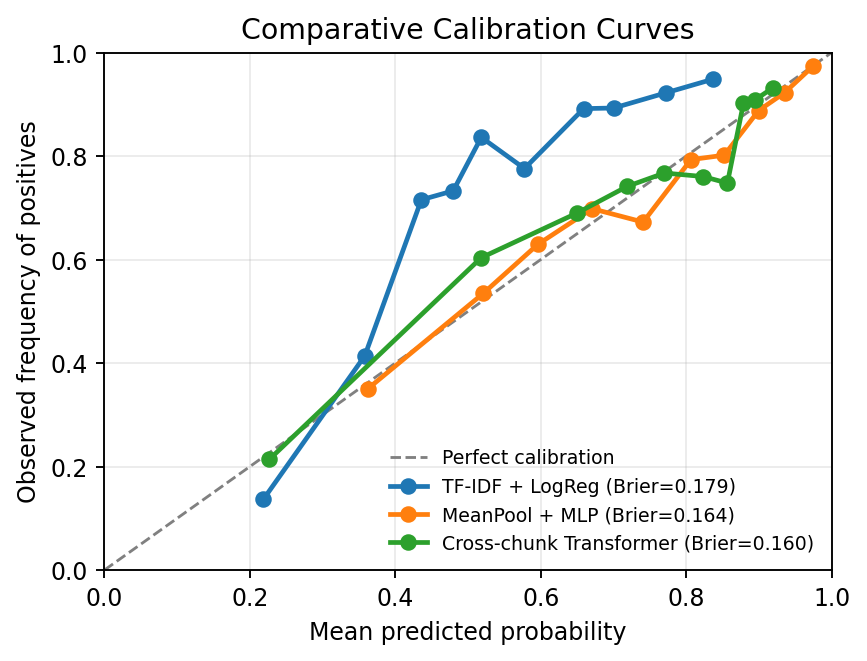
\includegraphics[width=0.94\linewidth]{figures/calibration_curve_cv.png}
  \caption{Curvas comparativas de calibración a partir de predicciones agregadas fuera de pliegue para TF--IDF + regresión logística, Promedio + MLP y el transformer entre fragmentos. La diagonal representa la calibración perfecta. El ordenamiento y la calibración no coinciden: el transformer se mantiene más próximo a una señal probabilística útil y calibrada, mientras que TF--IDF es más sólido como modelo de ordenamiento que como estimador de probabilidades.}
  \label{fig:calibration}
\end{figure}

\begin{figure}[t]
  \centering
  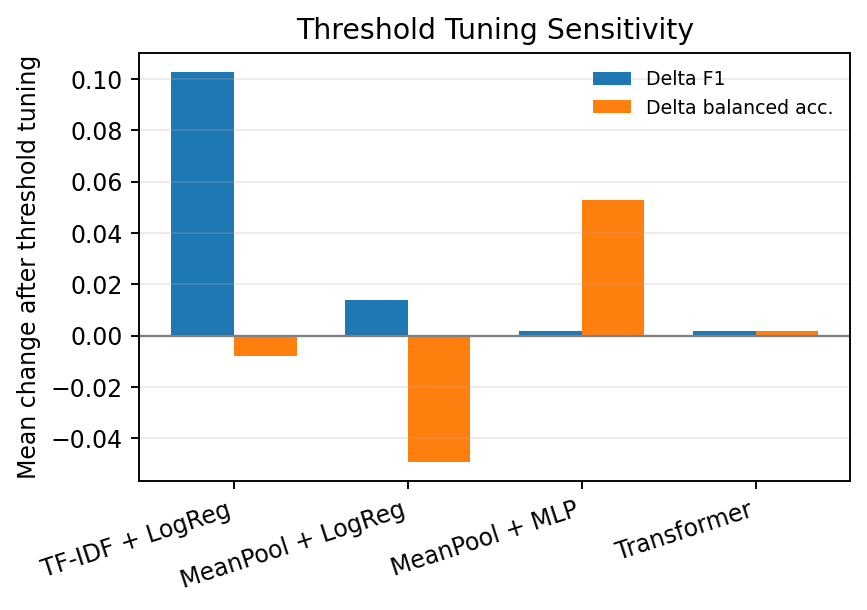
\includegraphics[width=0.94\linewidth]{figures/threshold_sensitivity_comparison.png}
  \caption{Cambio medio en F1 y exactitud balanceada del pliegue de prueba después de sustituir el umbral predeterminado de $0.5$ por el umbral que maximiza F1 en una partición interna de validación. El ajuste mejora considerablemente el F1 de TF--IDF + regresión logística, presenta efectos mixtos en los modelos con promedio y apenas modifica el transformer entre fragmentos, lo que indica una mayor estabilidad del punto operativo.}
  \label{fig:threshold-sensitivity}
\end{figure}
